
\documentclass[final]{beamer}

\usepackage[scale=1.24]{beamerposter} % Use the beamerposter package for laying out the poster

\usetheme{confposter} % Use the confposter theme supplied with this template

\setbeamercolor{block title}{fg=ngreen,bg=white} % Colors of the block titles
\setbeamercolor{block body}{fg=black,bg=white} % Colors of the body of blocks
\setbeamercolor{block alerted title}{fg=white,bg=dblue!70} % Colors of the highlighted block titles
\setbeamercolor{block alerted body}{fg=black,bg=dblue!10} % Colors of the body of highlighted blocks
% Many more colors are available for use in beamerthemeconfposter.sty

%-----------------------------------------------------------
% Define the column widths and overall poster size
% To set effective sepwid, onecolwid and twocolwid values, first choose how many columns you want and how much separation you want between columns
% In this template, the separation width chosen is 0.024 of the paper width and a 4-column layout
% onecolwid should therefore be (1-(# of columns+1)*sepwid)/# of columns e.g. (1-(4+1)*0.024)/4 = 0.22
% Set twocolwid to be (2*onecolwid)+sepwid = 0.464
% Set threecolwid to be (3*onecolwid)+2*sepwid = 0.708

\newlength{\sepwid}
\newlength{\onecolwid}
\newlength{\twocolwid}
\newlength{\threecolwid}
\setlength{\paperwidth}{48in} % A0 width: 46.8in
\setlength{\paperheight}{36in} % A0 height: 33.1in
\setlength{\sepwid}{0.024\paperwidth} % Separation width (white space) between columns
\setlength{\onecolwid}{0.22\paperwidth} % Width of one column
\setlength{\twocolwid}{0.464\paperwidth} % Width of two columns
\setlength{\threecolwid}{0.708\paperwidth} % Width of three columns
\setlength{\topmargin}{-0.5in} % Reduce the top margin size
%-----------------------------------------------------------

\usepackage{graphicx}  % Required for including images

\usepackage{booktabs} % Top and bottom rules for tables

%----------------------------------------------------------------------------------------
%   TITLE SECTION 
%----------------------------------------------------------------------------------------

\title{THUPost} % Poster title

\author{Miao Ren, Dichen Qian, Fengmin Zhu} % Author(s)

\institute{2016} % Institution(s)

%----------------------------------------------------------------------------------------

\begin{document}

\addtobeamertemplate{block end}{}{\vspace*{2ex}} % White space under blocks
\addtobeamertemplate{block alerted end}{}{\vspace*{2ex}} % White space under highlighted (alert) blocks

\setlength{\belowcaptionskip}{2ex} % White space under figures
\setlength\belowdisplayshortskip{2ex} % White space under equations

\begin{frame}[t] % The whole poster is enclosed in one beamer frame

\begin{columns}[t] % The whole poster consists of three major columns, the second of which is split into two columns twice - the [t] option aligns each column's content to the top

    \begin{column}{\sepwid}\end{column} % Empty spacer column

    \begin{column}{\onecolwid} % The first column

%----------------------------------------------------------------------------------------
%   OBJECTIVES
%----------------------------------------------------------------------------------------

        \begin{alertblock}{Objectives}
        What is THUPost?
        \begin{itemize}
        \item Second-hand goods market.
        \item Only served for THU students.
        \item Easy way for sharing and exchanging goods information.
        \end{itemize}

        \end{alertblock}

%----------------------------------------------------------------------------------------
%   QUICK REVISION
%----------------------------------------------------------------------------------------

        \begin{block}{Register}
        THUPost only server for students in Tsinghua University. As the university official authentication interface is too difficult to apply, THUPost use email of Tsinghua University to make authentication.

        % 这里搞一张图片注册界面
        \end{block}
        \begin{block}{Home}
        The home page of THUPost will show most functions. 

        The left side bar will lead to 4 diffrent and most common types of goods selled in university which are digital device, clothers, daily uses and books. Users can use this to select what things they want.

        From the top bar users can search products by enter some key words. THUPost will search the database to find the corresbonding goods and show them to the user.

        Users can also change their profile and check out what they selled and what they buyed both.

        The center of home page will show the most recent goods. These goods are selected by system based on its information.

        %这里来一张Home的截图
        % \begin{figure}
        % % \includegraphics[width=0.3\linewidth]{left_side_bar.png}
        % \caption{Left side bar}
        % \end{figure}

        % \textbf{Forms of Quadratic Function}
        % \begin{itemize}
        % \item $f(x) = ax^2+bx+c$ is called the \textbf{standard form}.
        % \item $f(x) = a(x-x_1)(x-x_2)$ is called the \textbf{factored form}, where $x_1$ and $x_2$ are the roots of the quadratic function.
        % \item $f(x) = a(x-h)^2+k$ is called the \textbf{vertex form}.
        % \end{itemize}

        % \textbf{Delta $\Delta$}\\*
        % $\Delta$ determines tells us how many solutions quadratic equation have:
        % $$\text{number of solutions}=
        % \begin{cases}
        % 2 &\text{when } \Delta > 0\\
        % 1 &\text{when } \Delta = 0\\
        % 0 &\text{when } \Delta < 0
        % \end{cases}
        % $$


        % \textbf{The Quadratic Formula}
        % $$x = \frac{-b\pm \sqrt{\Delta}}{2a}$$

        % \textbf{Graph of Quadratic Function}

        \end{block}

        \begin{figure}
        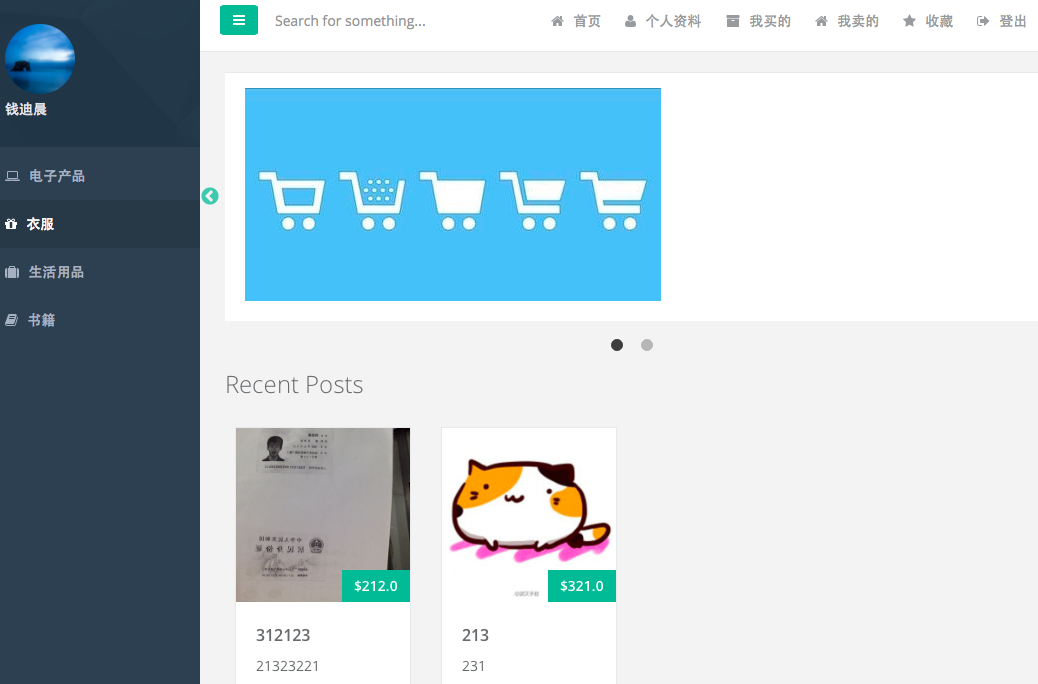
\includegraphics[width=1\linewidth]{home.png}
        \caption{home page}
        \end{figure}


%------------------------------------------------

% \begin{figure}
% 
\includegraphics[width=0.8\linewidth]{1.jpg}
% \caption{Graph of $f(x)=ax^2|_{\{0.1, 0.3, 1.0, 3.0\}}$}
% \end{figure}

%----------------------------------------------------------------------------------------

    \end{column} % End of the first column

    \begin{column}{\sepwid}\end{column} % Empty spacer column

    \begin{column}{\onecolwid} % Begin a column which is two columns wide (column 2)
% \begin{column}{\twocolwid} % Begin a column which is two columns wide (column 2)

% \begin{columns}[t,totalwidth=\twocolwid] % Split up the two columns wide column

% \begin{column}{\onecolwid}\vspace{-.6in} % The first column within column 2 (column 2.1)

%----------------------------------------------------------------------------------------
%   MATERIALS
%----------------------------------------------------------------------------------------
        \begin{block}{Information exchange}
        THUPost don't supply mail function for two purpose. 
        \begin{enumerate}
        \item Users don't spend too much time on THUPost, so they might forget to check out whether goods have been selled.
        \item Wechat and mail have better interaction than station letter.
        \end{enumerate}

        Instead THUPost need user to submit its Wechat ID or mobile phone so that sellers and buyers can exchange their ideas.


        \end{block}

        \begin{figure}
        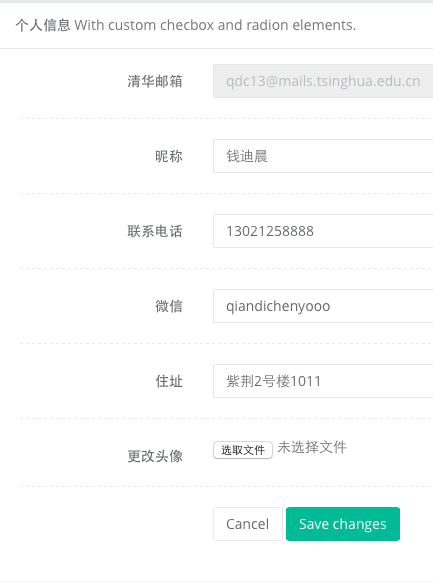
\includegraphics[width=0.4\linewidth]{information.png}
        \caption{user information}
        \end{figure}


        \begin{block}{Notification}
            Once the user create an order, he/she can notify the seller at once, either sending an email
            or a text message, by simply clicking the button.

        \end{block}



%----------------------------------------------------------------------------------------

    \end{column} % End of column 2.1
    \begin{column}{\sepwid}\end{column} % Empty spacer column
    \begin{column}{\onecolwid}\vspace{-.6in} % The second column within column 2 (column 2.2)
    

        \begin{block}{Backend \& Frontend}
        THUPost select several develop kit.
        \begin{enumerate}
        \item Ruby on Rails 2.3.1.
        \item Bootstrp
        \item MySQL
        \item jQuery
        \end{enumerate}

        Most html will produced by ROR erb file, in addition backend provide several API for frontend to use. This will drastically increase the interaction for user like.

        We select ActiveModel as the ROM class connecting with the database, it's really wonderful for this ROM skill interacting with database, convinient and efficient.

        We have four main models in database.
        \begin{enumerate}
        \item User, represents a user.
        \item Product, represents a goods to be selled.
        \item Order, represents one order between seller and buyer.
        \item Collection, represents the goods that one specific user collect.
        \end{enumerate}
        Based on these models, it's easy to manage our data in database.
        \end{block}

        \begin{block}{plugin}
            In order to achieve our goal providing good interaction for users, we use several fantastic plugin.
            \begin{enumerate}
            \item Devise, fantastic plugin managing login logout.
            \item Paperclip, providing useful image managing and resize function. It can also change the pixis of image into suitable size.
            \item Sweetalert, a useful function to draw the alert window.
            \end{enumerate}
        \end{block}
%----------------------------------------------------------------------------------------
%   P
%----------------------------------------------------------------------------------------


%----------------------------------------------------------------------------------------

    \end{column} % End of column 2.2
    % \begin{column}{\sepwid}\end{column} % Empty spacer column
        
    \begin{column}{\onecolwid}
        Fourth column.
    \end{column}
\end{columns} % End of the split of column 2 - any content after this will now take up 2 columns width

%----------------------------------------------------------------------------------------
%   IMPORTANT To REMEMBER
%----------------------------------------------------------------------------------------



%----------------------------------------------------------------------------------------

% \begin{columns}[t,totalwidth=\twocolwid] % Split up the two columns wide column again

%     \begin{column}{\onecolwid} % The first column within column 2 (column 2.1)

% %----------------------------------------------------------------------------------------
% %   EXAMPLE OF FACTORISATION
% %----------------------------------------------------------------------------------------

% %----------------------------------------------------------------------------------------

%     \end{column} % End of column 2.1

%     \begin{column}{\onecolwid} % The second column within column 2 (column 2.2)

% %----------------------------------------------------------------------------------------
% %   PROOF OF VIETA'S FORMULAS
% %----------------------------------------------------------------------------------------


% %----------------------------------------------------------------------------------------

%     \end{column} % End of column 2.2

% \end{columns} % End of the split of column 2

% % \end{column} % End of the second column

% \begin{column}{\sepwid}\end{column} % Empty spacer column

% \begin{column}{\onecolwid} % The third column

% %----------------------------------------------------------------------------------------
% %   CONCLUSION
% %----------------------------------------------------------------------------------------


% %----------------------------------------------------------------------------------------
% %   ACKNOWLEDGEMENTS
% %----------------------------------------------------------------------------------------


% %----------------------------------------------------------------------------------------

% \end{column} % End of the third column

% \end{columns} % End of all the columns in the poster

\end{frame} % End of the enclosing frame

\end{document}
